\begin{frame}{Contents}
  \begin{itemize}
  \item $d(K^-, n \pi^+ \pi^-)"n"$ events
    \begin{enumerate}
    \item $K^- d \rightarrow \pi^{\mp} \Sigma^{\pm}_{backward} n_{forward}$ $\rightarrow$ Main signal in my analysis
    \item $K^- d \rightarrow n_{detect} K^0 n_{missing}$\\
      2-step like events was observed (before meeting). \\
      What reaction happened in $d(K^-, n)$ reaction. $\leftarrow$ Today theme
    \item $K^- d \rightarrow \Sigma_{fowrad}^{\pm} \pi^{\mp} n_{missing}$  Negligible small
    \end{enumerate}  
  \end{itemize}

  \begin{tabular}{cc}
    \begin{minipage}{0.5\hsize}
      \begin{figure}
        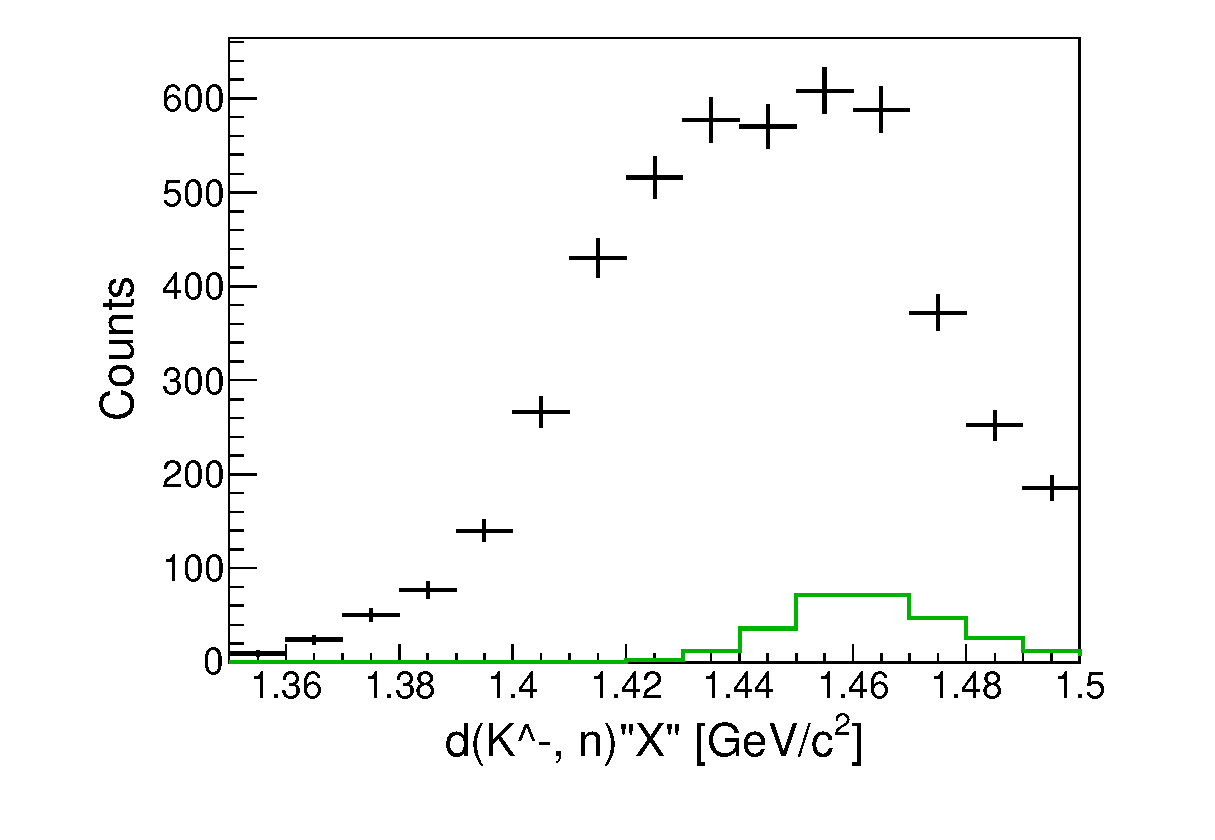
\includegraphics[width=3cm]{../pic/Run78//KN_ana_NC170_2sigma//KN_MM_woAll.eps}
      \end{figure}
      \vspace{-3mm}
      \tiny
      \centering
      $d(K^-, n)"\pi^{\mp}\Sigma^{\pm}"$ like events.\\
      $K^0$ and $\Sigma^{\pm}_{forward}$ were rejected.\\
      Contaminations was estimated by template fitting of\\ invariant masses, $\pi^+ \pi^-, n \pi^+, n \pi^-$.
    \end{minipage}

    \begin{minipage}{0,5\hsize}
      \begin{figure}
        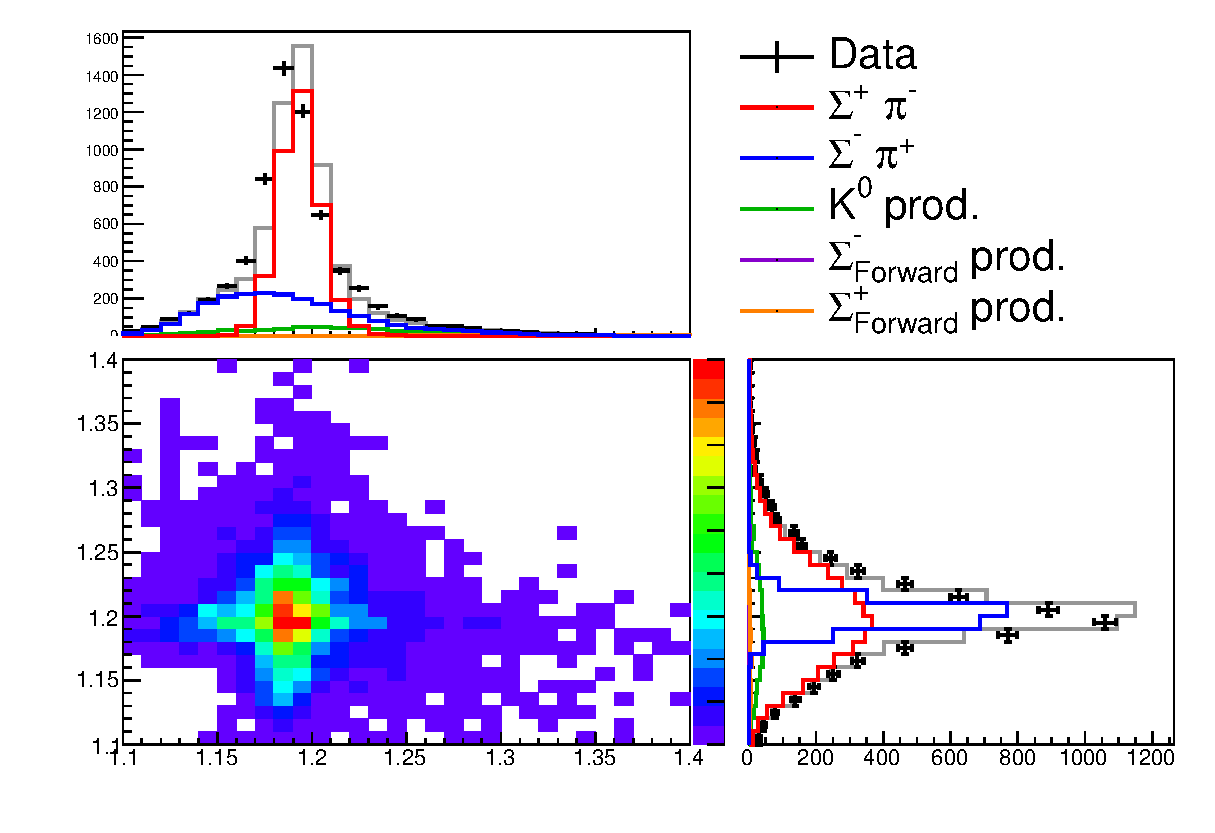
\includegraphics[width=3.5cm]{../pic/Run78/KN_ana_NC170_2sigma/KNpim_KNpip_MM.eps}        
      \end{figure}
      \vspace{-3mm}
      \tiny
      \centering
      $\textcolor{red}{d(K^-, n)"\pi^-\Sigma^+"}$ and $\textcolor{blue}{d(K^-, n)"\pi^+\Sigma^-"}$ modes \\
      were separated by $d(K^-, n \pi^{\mp})"\Sigma^{\pm}"$ missing masses.\\
      This separation was performed bin-by-bin of $\pi^{\mp}\Sigma^{\pm}$
    \end{minipage}
  \end{tabular}
\end{frame}
